\section{Kapitel 4}
%TODO
\subsection{Atraktorbereich und Separatrizen}
Haben wir ein autonomes System mit Anfangswertproblem. Die Gesamtheit aller Punkte des Phasenraums - die als Anfangsbedingung gewählt - zu einer Trajektorie führen, welche dann gegen einen speziellen Punkt konvergiert, heisst Atraktorbereich des Punktes. 
Die Ränder, welche diese Bereiche trennen, heissen Separatrizen. 
Im Bild sehen wir zwei Atraktorbereiche, welche durch die beiden blauen Kurven (die Separatrizen) getrennt sind. 
Startet man innerhalb der Blase, so konvergiert man gegen den Punkt (0,0) ansonsten gegen den Punkt (1,-2). 
\begin{minipage}[h]{0.35\textwidth}
	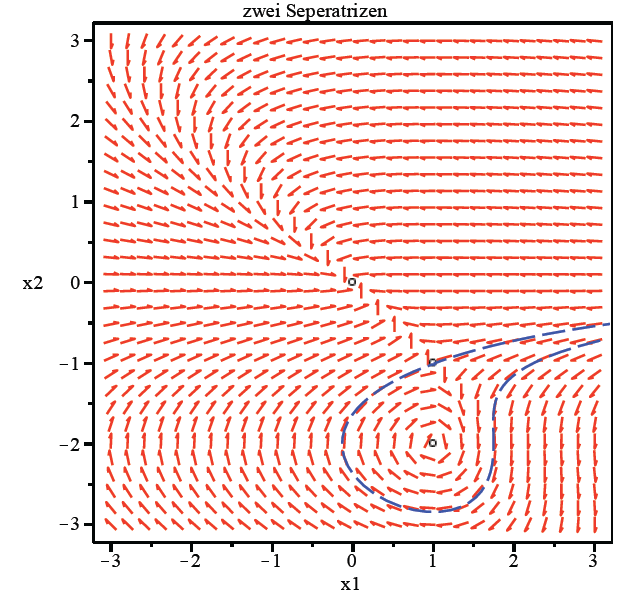
\includegraphics[width=1.0\textwidth]{images/Atraktorbereich.png}
\end{minipage}
\subsection{Fast lineare Systeme, Jakobi-Matrix}
Ein System ist fast linear, wenn die Jacobimatrix $J_f$ regulär ist $det(J_f)\neq 0$. \\
1.Schritt: DGL in Form bringen:\\ 
$x'_1(t) = f_1(t) = x_2(t)$\\
$x'_2(t) = f_2(t) = -q(t)x_1(t)-p(t)x_2(t)+g(t)$\\
2.Schritt: Jacobi Matrix berechnen:\\
\begin{equation*}
	J_f(x) =    
	\begin{vmatrix} 
	        \frac{\partial f_1}{\partial x_1} & \frac{\partial f_1}{\partial x_2}\\ 
	        \frac{\partial f_2}{\partial x_1} & \frac{\partial f_2}{\partial x_2}\\   
	\end{vmatrix}
\end{equation*}
3. Schritt: Kritische Punkte berechnen (Ableitungen Null setzen...) $\rightarrow \epsilon_1, \epsilon_2...$\\
4. Schritt: Jeden kritischen Punkt separat in die Jacobimatrix einsetzen\\
5. Schritt: Anschliessen für jede Jacobimatrix die Eigenwerte ausrechnen \\
6. Schritt: Stabilität nach folgender Tabelle beurteilen\\
\begin{minipage}[h]{0.7\textwidth}
	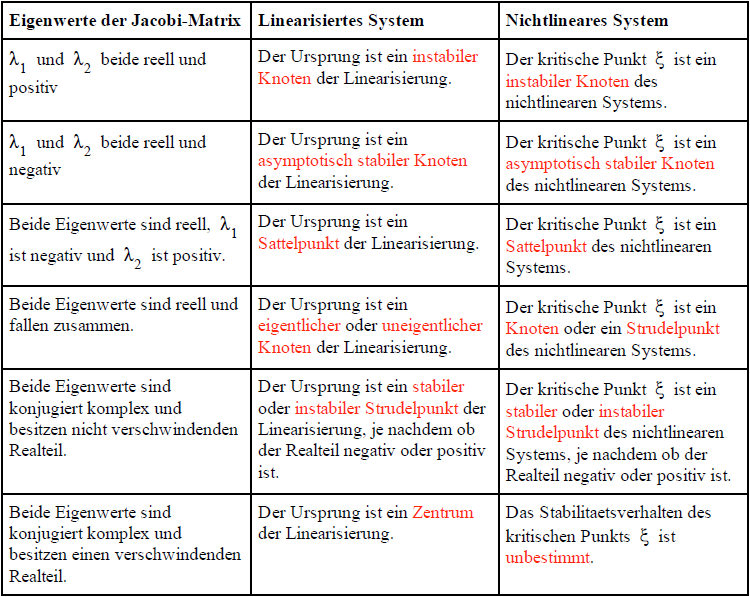
\includegraphics[width=1.0\textwidth]{images/JacobiTabelle.png}
\end{minipage}

\subsection{Bilanzieren}
\begin{minipage}[h]{0.7\textwidth}
	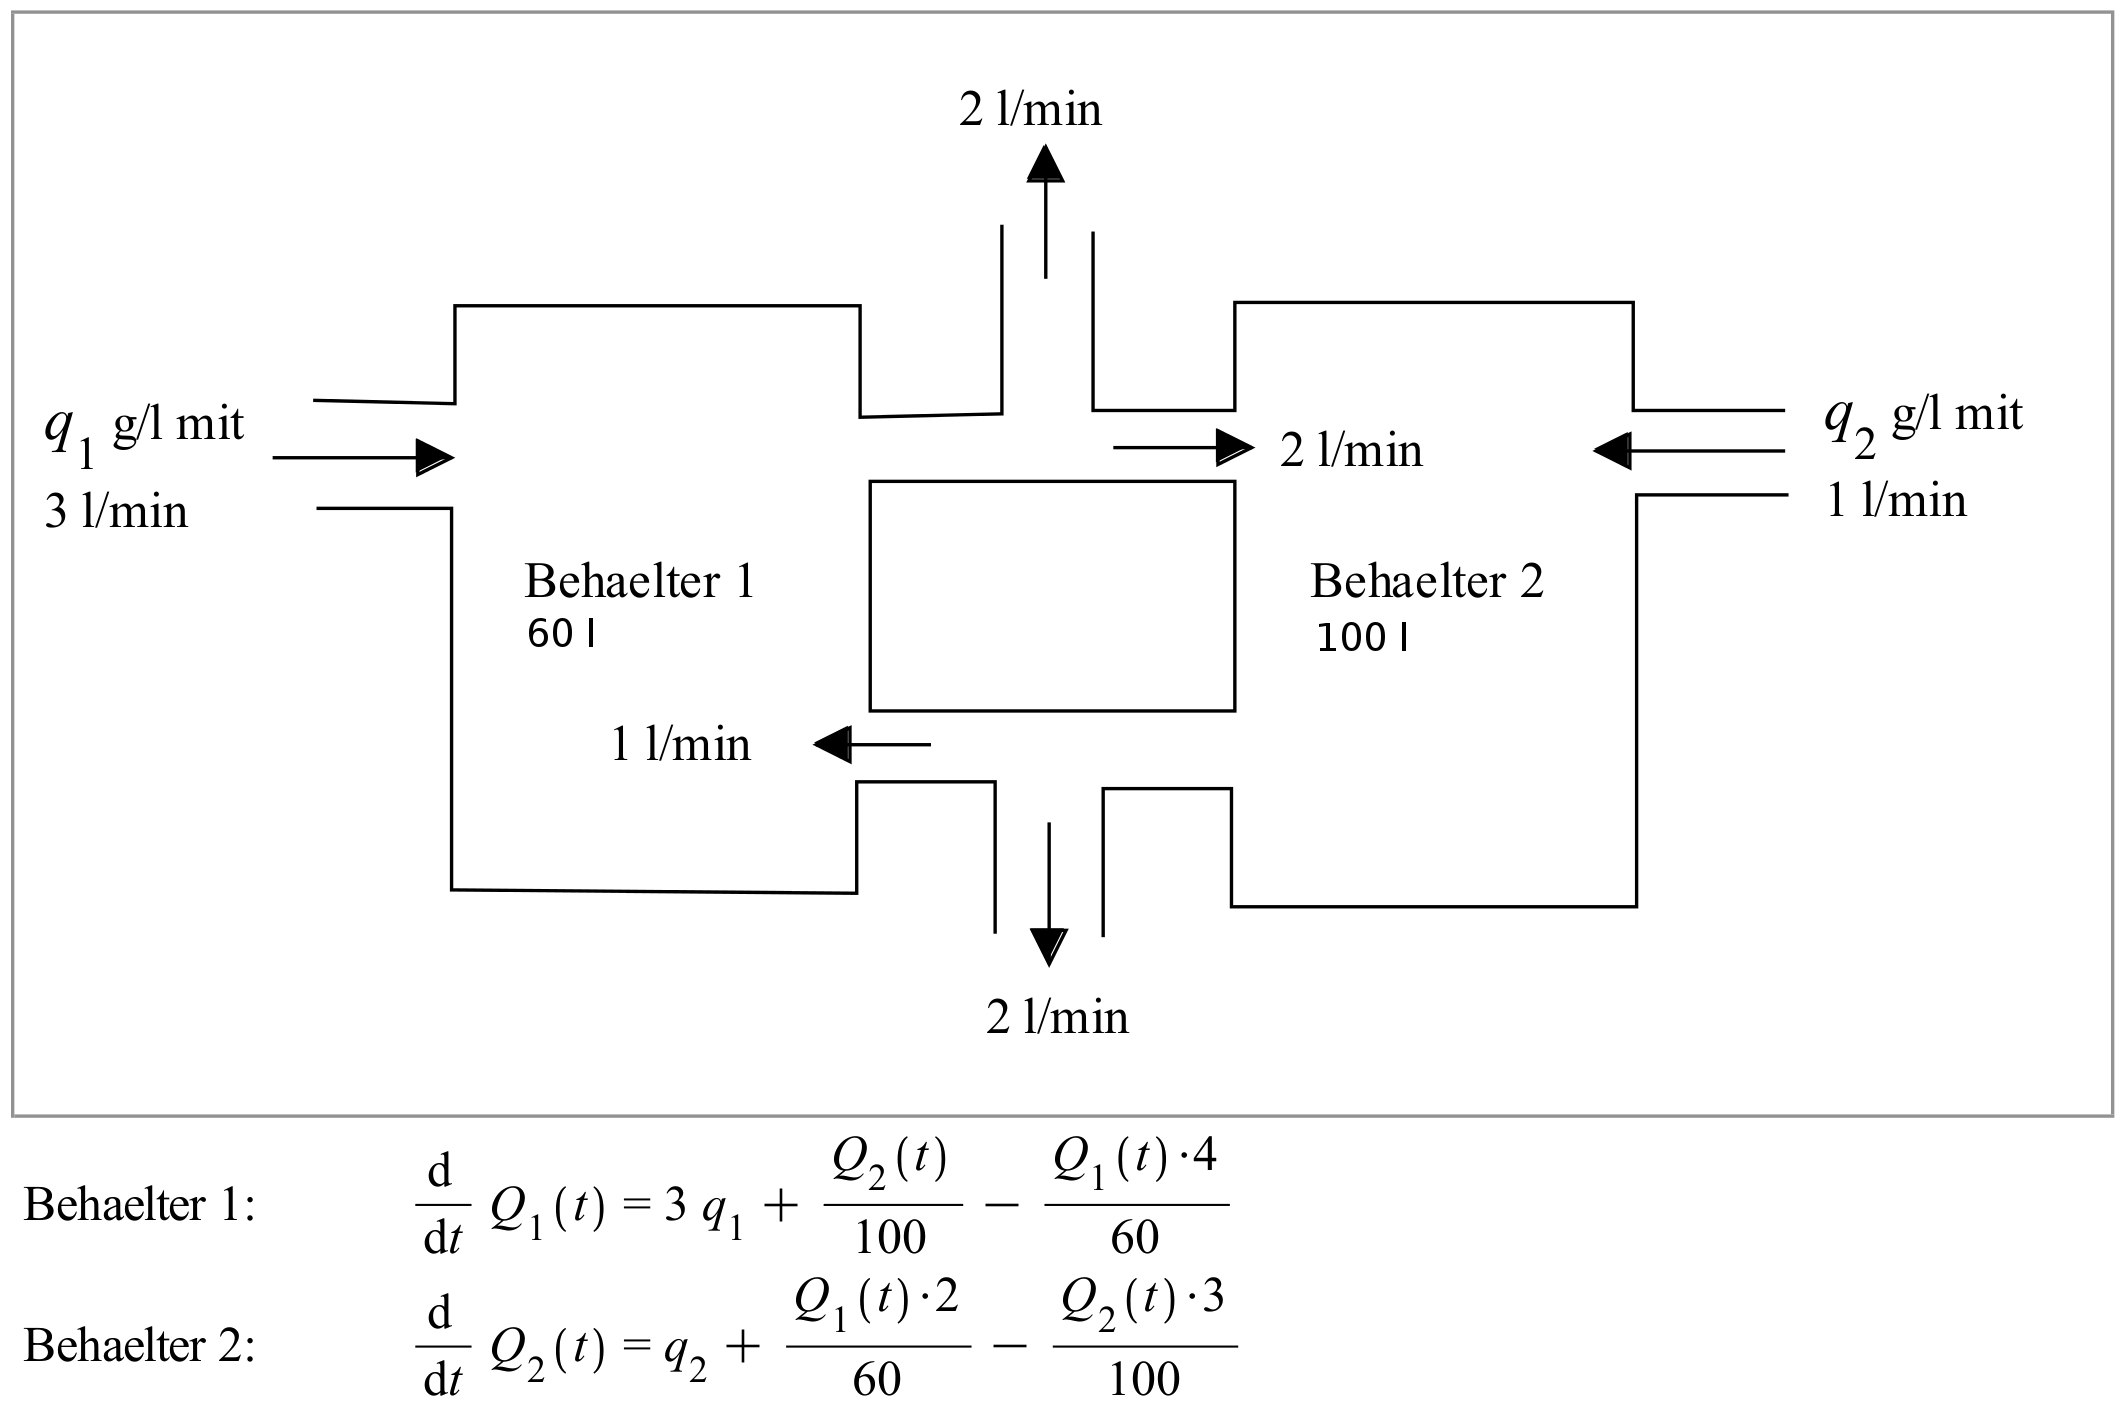
\includegraphics[width=1.0\textwidth]{images/Bilanzieren.png}
\end{minipage}

\subsection{Konkurrenz-Modell, Räuber-Beute-Modell, Grenzzyklen}
Aus Zeitgründen konnten wir diese Themen nicht auch noch bearbeiten. Dankbar nehmen wir hier einen Teil aus der ZF von Christoph Danedliker. \\
\begin{minipage}[h]{1\textwidth}
	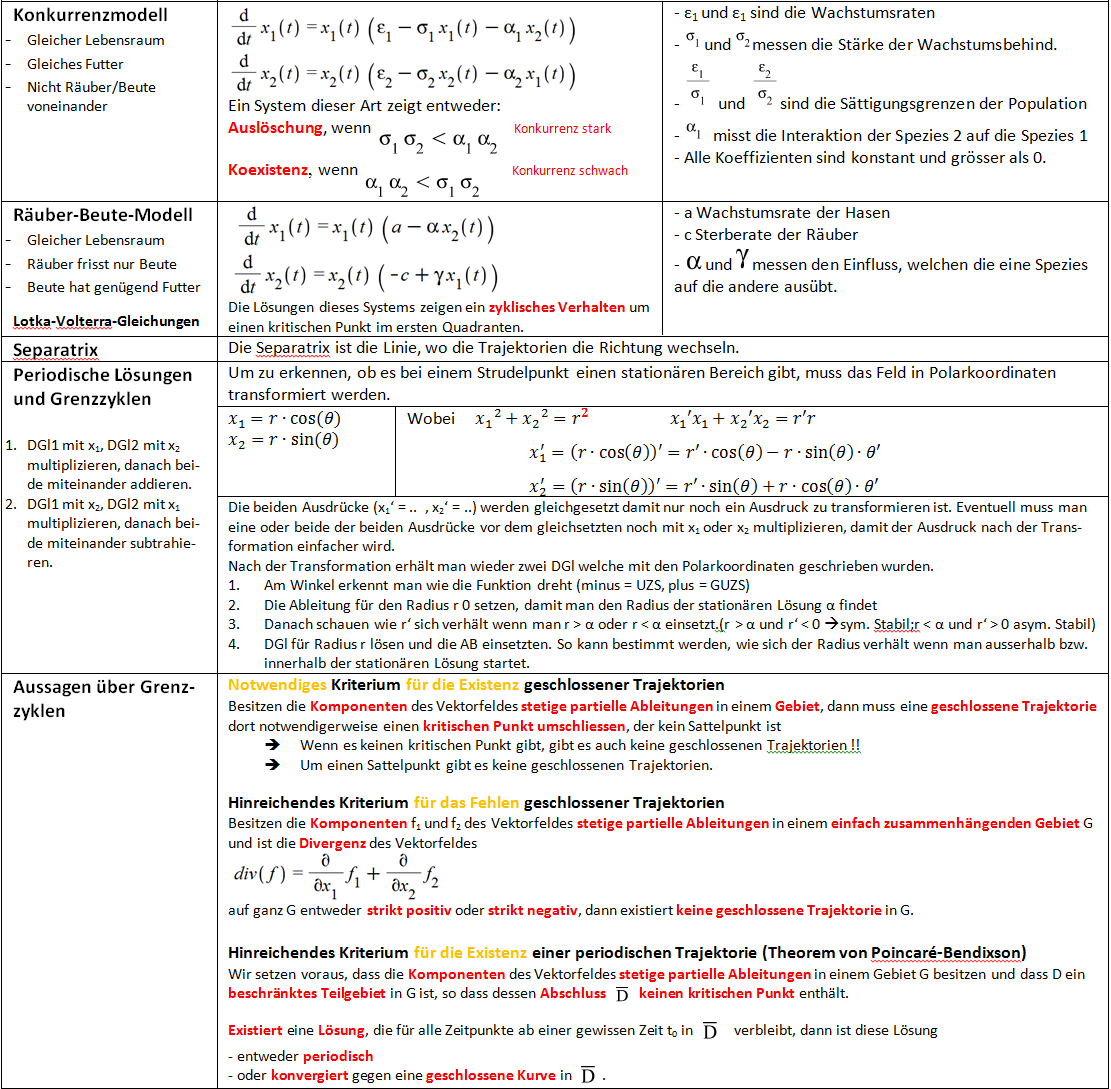
\includegraphics[width=1.0\textwidth]{images/Rest.png}
\end{minipage}
